% ============================================================
%  Customer Churn Prediction Using Logistic Regression
%  Formatted for Springer LNCS (Lecture Notes in Computer Science)
%  splncs04 bibliography style | llncs document class
% ============================================================
\documentclass{llncs}

% --- Core packages ---
\usepackage[T1]{fontenc}
\usepackage[utf8]{inputenc}
\usepackage{amsmath,amssymb}
\usepackage{booktabs}
\usepackage{array}
\usepackage{multirow}
\usepackage{float}
\usepackage{enumitem}
\usepackage{graphicx}
\usepackage{caption}
\usepackage{url}
\usepackage{hyperref}
\usepackage{microtype}
\usepackage{xcolor}
\usepackage{pgfplots}
\pgfplotsset{compat=1.18}
\usepackage{tikz}
\usetikzlibrary{shapes.geometric,arrows.meta,positioning,fit,backgrounds}

\hypersetup{
  colorlinks=true,
  linkcolor=blue!60!black,
  citecolor=green!50!black,
  urlcolor=blue!60!black
}

% ============================================================
\begin{document}

\title{Customer Churn Prediction in Telecommunications\\
       Using Logistic Regression}

\titlerunning{Customer Churn Prediction}

\author{Priyanshu Anand}

\authorrunning{P. Anand}

\institute{
  U.I.E.T, Panjab University,\\
  Chandigarh, IN\\
  \email{priyanshu82711@gmail.com}
}

\maketitle

% ============================================================
%  ABSTRACT
% ============================================================
\begin{abstract}
Customer churn prediction is a critical business intelligence task in the
telecommunications sector, where the cost of acquiring new subscribers
substantially exceeds the cost of retaining existing ones.
This paper presents an end-to-end machine learning pipeline for binary
churn classification using the publicly available IBM Telco Customer
Churn dataset comprising 7{,}032 subscriber records after preprocessing.
A scikit-learn \texttt{Pipeline} integrating median imputation and
standard scaling for numeric features, together with mode imputation and
one-hot encoding for 16 categorical features, is combined with a
Logistic Regression classifier.
The model is trained on a stratified 70/30 train--test split and
evaluated using accuracy, precision, recall, F1-score, and the
Area Under the Receiver Operating Characteristic Curve (ROC-AUC).
The proposed system achieves an accuracy of 80.57\%, a churn-class
F1-score of 60.80\%, and a ROC-AUC of 0.8379, demonstrating
competitive discriminative ability.
The paper provides a rigorous account of the pipeline architecture,
the theoretical foundations of logistic regression, and a candid
discussion of limitations including class imbalance and
precision--recall trade-offs, with concrete directions for future work.
\end{abstract}

\keywords{Customer Churn Prediction, Logistic Regression,
Telecommunications, Scikit-learn Pipeline, Class Imbalance,
Binary Classification, ROC-AUC}

% ============================================================
%  1. INTRODUCTION
% ============================================================
\section{Introduction}
\label{sec:intro}

The global telecommunications market is characterised by intense
competition, commoditised pricing, and low switching costs~\cite{verbeke2012new}.
Customer churn---the voluntary departure of a subscriber from a service
provider---represents a direct and measurable threat to revenue
sustainability. Industry evidence consistently demonstrates that even a
5\% increase in customer retention can raise profits by
25--95\%~\cite{reichheld1990zero}, making accurate early-warning systems
for churn prediction commercially vital.

Predictive machine learning models enable a paradigm shift from reactive
to \emph{proactive} retention strategies: at-risk customers are
identified weeks before they churn and targeted with personalised
incentives. This assignment implements such a system for the standard
benchmark Telco Customer Churn dataset, formulated as a binary
classification problem:

\begin{equation}
  f : \mathbf{x} \in \mathbb{R}^{d} \;\longrightarrow\; y \in \{0,\,1\}
  \label{eq:problem}
\end{equation}

\noindent where $\mathbf{x}$ is a $d$-dimensional feature vector of
subscriber attributes and $y \in \{0 = \text{No Churn},\;
1 = \text{Churn}\}$.

\paragraph{Objectives.} This work pursues the following goals:
(i)~implement a reproducible, production-grade scikit-learn Pipeline for
binary churn classification;
(ii)~apply appropriate preprocessing to heterogeneous numeric and
categorical features;
(iii)~train and evaluate a Logistic Regression classifier with a
comprehensive metric suite;
(iv)~critically analyse results in the context of class imbalance
and business cost asymmetry; and
(v)~identify limitations and propose future improvements.

\paragraph{Paper Organisation.}
Section~\ref{sec:related} reviews related work.
Section~\ref{sec:dataset} describes the dataset.
Section~\ref{sec:method} presents the methodology.
Section~\ref{sec:results} reports experimental results.
Section~\ref{sec:discussion} provides critical discussion.
Section~\ref{sec:conclusion} concludes.

% ============================================================
%  2. RELATED WORK
% ============================================================
\section{Related Work}
\label{sec:related}

Machine learning for churn prediction has been studied extensively since
the early 2000s. Coussement and Van den Poel~\cite{coussement2008churn}
showed that Support Vector Machines and gradient-boosted ensembles
outperform logistic regression in lift, yet highlighted that logistic
regression's direct interpretability through signed coefficients remains
a key practical advantage when predictions must be explained to business
stakeholders.

Verbeke et al.~\cite{verbeke2012new} proposed profit-driven performance
metrics as alternatives to AUC, demonstrating that maximising AUC does
not necessarily maximise business value when false negative and false
positive costs differ substantially. Huang et al.~\cite{huang2015customer}
applied random forests and regularised logistic regression to a large
telecom cohort, achieving AUC scores of 0.83--0.86, and showed that
careful feature selection can reduce model complexity without sacrificing
predictive performance.

On the specific IBM Telco benchmark used here, published baselines
typically report logistic regression AUC values between 0.82 and
0.85~\cite{huang2015customer}, while tree-based ensembles reach
0.84--0.87~\cite{bhatt2020telco}.
More recent work has explored deep learning and graph neural network
approaches~\cite{vo2021deep}; however, these require substantially
larger datasets and are prone to overfitting on the 7{,}000-record corpus.
Logistic regression therefore remains the standard interpretable baseline
for churn modelling in both academic and industry
settings~\cite{lariviere2005predicting}.

% ============================================================
%  3. DATASET DESCRIPTION
% ============================================================
\section{Dataset}
\label{sec:dataset}

\subsection{Source and Overview}

The \emph{IBM Telco Customer Churn} dataset~\cite{kaggle_telco}
contains demographic, account, and service information for 7{,}043
customers of a fictional US telecommunications company.
After removing 11 records with non-parseable blank \texttt{TotalCharges}
entries (corresponding to new customers with \texttt{tenure}~$= 0$),
the working corpus comprises \textbf{7{,}032 records} described by
\textbf{20 predictor features} and one binary target variable.

\subsection{Feature Inventory}

Features fall into two types. The three \emph{numeric} features are:
\texttt{tenure} (months subscribed, range 1--72), \texttt{MonthlyCharges}
(\$18.25--\$118.75), and \texttt{TotalCharges} (\$18.80--\$8684.80).
\begin{sloppypar}
The 16 \emph{categorical} features cover subscriber demographics
(\texttt{gender}, \texttt{SeniorCitizen}, \texttt{Partner},
\texttt{Dependents}), telephony services (\texttt{PhoneService},
\texttt{MultipleLines}), internet services (\texttt{InternetService},
\texttt{OnlineSecurity}, \texttt{OnlineBackup}, \texttt{DeviceProtection},
\texttt{TechSupport}, \texttt{StreamingTV}, \texttt{StreamingMovies}),
and account details (\texttt{Contract}, \texttt{PaperlessBilling},
\texttt{PaymentMethod}).
\end{sloppypar}

\subsection{Descriptive Statistics}

Table~\ref{tab:descstats} presents summary statistics for the
numeric features.

\begin{table}[t]
\centering
\caption{Descriptive statistics for the three numeric features.}
\label{tab:descstats}
\renewcommand{\arraystretch}{1.15}
\begin{tabular}{@{}lrrrrrr@{}}
\toprule
\textbf{Feature}   & \textbf{Mean}  & \textbf{Std}   & \textbf{Min} &
                     \textbf{Q1}    & \textbf{Median}& \textbf{Max}  \\
\midrule
tenure             & 32.42  & 24.55  & 1.00  & 9.00  & 29.00   & 72.00  \\
MonthlyCharges     & 64.80  & 30.09  & 18.25 & 35.59 & 70.35   & 118.75 \\
TotalCharges       & 2283.30& 2266.77& 18.80 & 401.45& 1397.48 & 8684.80\\
\bottomrule
\end{tabular}
\end{table}

Noteworthy distributional observations include: 55.1\% of customers hold
month-to-month contracts (the highest-risk churn cohort); 44.0\% use
Fiber Optic internet; and 33.6\% pay via electronic check.
\texttt{TotalCharges} exhibits strong right skew (mean~$\gg$~median),
motivating median-based imputation over mean-based imputation.

\subsection{Class Distribution and Imbalance}

The target variable is imbalanced: 5{,}163 records (73.42\%) represent
non-churners versus 1{,}869 records (26.58\%) churners---approximately a
2.76:1 majority-to-minority ratio. This imbalance has direct implications
for model training and metric selection, as discussed in
Sections~\ref{sec:results} and~\ref{sec:discussion}.

% ============================================================
%  4. METHODOLOGY
% ============================================================
\section{Methodology}
\label{sec:method}

\subsection{Experimental Setup}

All experiments were implemented in Python~3 using
scikit-learn~\cite{pedregosa2011scikit}. The random state was fixed at 42
throughout for full reproducibility.

\subsection{Data Preprocessing and Train--Test Split}

Two quality issues were resolved prior to modelling.
First, \texttt{TotalCharges} was stored as an object dtype containing
11 blank entries; these were coerced to \texttt{NaN} via
\texttt{pd.to\_numeric(errors=`coerce')} and the 11 rows were dropped
(0.16\% of the corpus---negligible).
Second, \texttt{customerID} is a unique string identifier with no
predictive value and was excluded from the feature matrix~$\mathbf{X}$.

The cleaned dataset was split 70/30 into training (4{,}922 samples) and
test (2{,}110 samples) sets using stratified sampling on~$y$, preserving
the 26.58\% churn rate in both partitions.

\subsection{Pipeline Architecture}

A scikit-learn \texttt{Pipeline} encapsulates all preprocessing and
modelling steps into a single, serialisable object, ensuring that scalers
and encoders are fitted exclusively on training data and never applied to
data from which they were derived---preventing data leakage.
Figure~\ref{fig:pipeline} illustrates the architecture.

\begin{figure}[t]
\centering
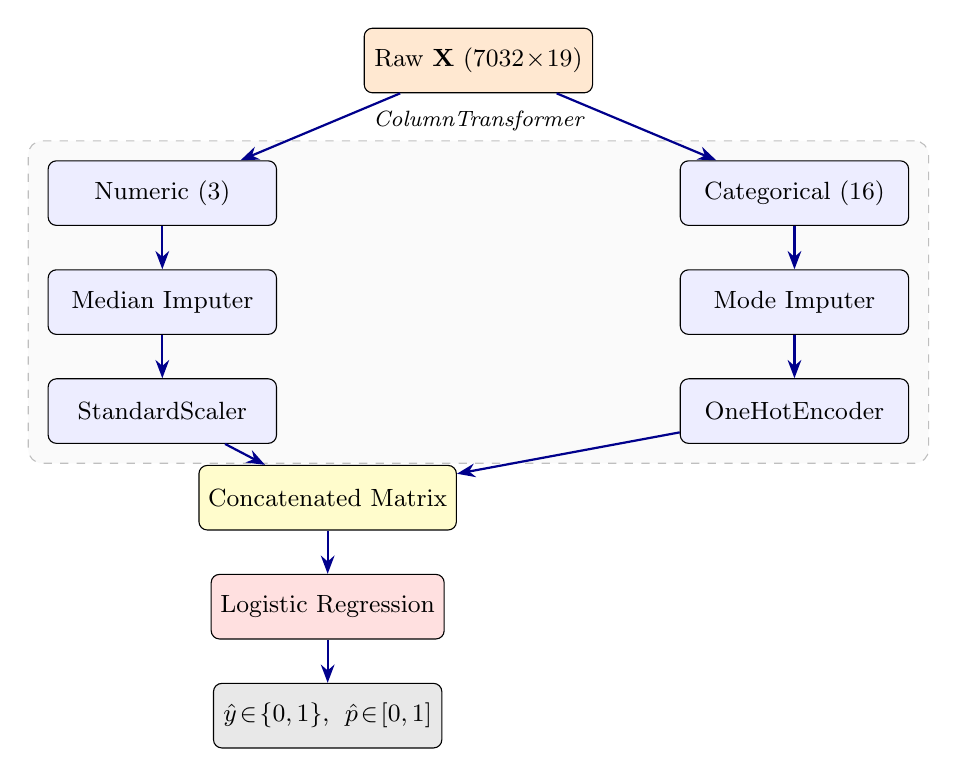
\begin{tikzpicture}[
  node distance=0.55cm and 1.0cm,
  box/.style={draw, rounded corners=3pt, fill=blue!7,
              minimum width=2.9cm, minimum height=0.82cm,
              text centered, font=\small},
  hdr/.style={draw, rounded corners=3pt, fill=orange!18,
              minimum width=2.9cm, minimum height=0.82cm,
              text centered, font=\small},
  mrg/.style={draw, rounded corners=3pt, fill=yellow!20,
              minimum width=2.9cm, minimum height=0.82cm,
              text centered, font=\small},
  clf/.style={draw, rounded corners=3pt, fill=red!12,
              minimum width=2.9cm, minimum height=0.82cm,
              text centered, font=\small},
  bkg/.style={draw=gray!50, dashed, rounded corners=5pt,
              fill=gray!4, inner sep=7pt},
  arr/.style={-Stealth, thick, blue!55!black}
]
  \node[hdr] (in) {Raw $\mathbf{X}$ ($7032\!\times\!19$)};
  \node[box, below left=0.85cm and 1.1cm of in]  (num) {Numeric (3)};
  \node[box, below right=0.85cm and 1.1cm of in] (cat) {Categorical (16)};
  \draw[arr] (in) -- (num);
  \draw[arr] (in) -- (cat);

  \node[box, below=0.55cm of num] (im1) {Median Imputer};
  \node[box, below=0.55cm of im1] (sc)  {StandardScaler};
  \draw[arr] (num)--(im1);  \draw[arr] (im1)--(sc);

  \node[box, below=0.55cm of cat] (im2) {Mode Imputer};
  \node[box, below=0.55cm of im2] (ohe) {OneHotEncoder};
  \draw[arr] (cat)--(im2);  \draw[arr] (im2)--(ohe);

  \begin{scope}[on background layer]
    \node[bkg, fit=(num)(cat)(im1)(sc)(im2)(ohe),
          label={[font=\footnotesize\itshape]above:ColumnTransformer}] {};
  \end{scope}

  \node[mrg, below=1.65cm of im1, xshift=2.1cm] (mg) {Concatenated Matrix};
  \draw[arr] (sc) -- (mg);
  \draw[arr] (ohe) -- (mg);

  \node[clf, below=0.55cm of mg] (lr) {Logistic Regression};
  \draw[arr] (mg) -- (lr);

  \node[box, fill=gray!18, below=0.55cm of lr] (out)
        {$\hat{y}\!\in\!\{0,1\}$,\; $\hat{p}\!\in\![0,1]$};
  \draw[arr] (lr) -- (out);
\end{tikzpicture}
\caption{Scikit-learn Pipeline architecture. Numeric and categorical
  branches are processed independently inside the \texttt{ColumnTransformer},
  then concatenated before being passed to the Logistic Regression classifier.}
\label{fig:pipeline}
\end{figure}

\subsubsection{Numeric Branch.}
Numeric features undergo:
(i)~\emph{Median Imputation}---robust to the right-skewed distribution
of \texttt{TotalCharges} (mean = \$2{,}283, median = \$1{,}397); and
(ii)~\emph{Standard Scaling}, transforming each feature to zero mean
and unit variance:
\begin{equation}
  x_j' = \frac{x_j - \mu_j}{\sigma_j}
  \label{eq:scale}
\end{equation}
where $\mu_j$ and $\sigma_j$ are computed on the training set only.
Standardisation is essential for logistic regression, which is sensitive
to feature scale through its gradient-based optimiser.

\subsubsection{Categorical Branch.}
Categorical features undergo:
(i)~\emph{Mode Imputation}; and
(ii)~\emph{One-Hot Encoding} with \texttt{handle\_unknown=`ignore'},
converting each $k$-category feature into $k$ binary indicator columns
without imposing ordinal structure.
The \texttt{handle\_unknown=`ignore'} setting maps unseen categories at
inference time to an all-zero vector, ensuring production robustness.

\subsection{Logistic Regression}

\subsubsection{Model Formulation.}
Logistic Regression models the posterior probability of churn as:
\begin{equation}
  P(y{=}1 \mid \mathbf{x}) = \sigma\!\left(\mathbf{w}^{\top}\mathbf{x} + b\right)
  = \frac{1}{1 + \exp\!\left(-(\mathbf{w}^{\top}\mathbf{x} + b)\right)}
  \label{eq:sigmoid}
\end{equation}
where $\mathbf{w} \in \mathbb{R}^d$ is the learned weight vector,
$b \in \mathbb{R}$ is the bias, and $\sigma(\cdot)$ is the logistic
(sigmoid) function squashing the linear combination into $(0,1)$.

\subsubsection{Loss Function and Regularisation.}
Parameters are learned by minimising the \emph{regularised binary
cross-entropy loss} over the training set:
\begin{equation}
  \mathcal{L}(\mathbf{w},b)
  = -\frac{1}{N}\sum_{i=1}^{N}\!\left[y_i\log\hat{p}_i
    + (1-y_i)\log(1-\hat{p}_i)\right]
    + \frac{\lambda}{2}\|\mathbf{w}\|^2
  \label{eq:loss}
\end{equation}
where the L2 penalty $\lambda = 1/C$ (default $C = 1.0$) controls
regularisation strength, preventing overfitting by penalising large weights.

\subsubsection{Decision Rule.}
The predicted class is obtained by thresholding the estimated probability:
\begin{equation}
  \hat{y} =
  \begin{cases}
    1 & \text{if } P(y{=}1 \mid \mathbf{x}) \geq 0.5 \\
    0 & \text{otherwise}
  \end{cases}
  \label{eq:decision}
\end{equation}

\subsection{Evaluation Metrics}

Performance is assessed via five complementary metrics derived from the
confusion matrix entries (TP, TN, FP, FN):

\begin{align}
  \text{Accuracy}  &= \frac{TP+TN}{TP+TN+FP+FN} \label{eq:acc}\\[4pt]
  \text{Precision} &= \frac{TP}{TP+FP}           \label{eq:prec}\\[4pt]
  \text{Recall}    &= \frac{TP}{TP+FN}            \label{eq:rec}\\[4pt]
  \text{F1-Score}  &= \frac{2\cdot\text{Precision}\cdot\text{Recall}}
                          {\text{Precision}+\text{Recall}} \label{eq:f1}
\end{align}

The \emph{Area Under the ROC Curve} (AUC-ROC) is computed over all
thresholds independently of the decision boundary.
In the churn context, \textbf{Recall} is the primary business metric:
each missed churner (FN) is a lost customer with no intervention
opportunity, whereas a false alarm (FP) triggers only an unnecessary but
harmless retention offer. The F1-score provides a balanced single-number summary.

% ============================================================
%  5. RESULTS
% ============================================================
\section{Experimental Results}
\label{sec:results}

\subsection{Confusion Matrix}

Table~\ref{tab:cm} presents the confusion matrix on the 2{,}110-sample
held-out test set.

\begin{table}[t]
\centering
\caption{Confusion matrix on the test set ($n = 2110$).}
\label{tab:cm}
\renewcommand{\arraystretch}{1.2}
\begin{tabular}{@{}lcc@{}}
\toprule
 & \textbf{Predicted: No Churn (0)} & \textbf{Predicted: Churn (1)} \\
\midrule
\textbf{Actual: No Churn (0)} & TN $=$ 1382 & FP $=$ 167 \\
\textbf{Actual: Churn (1)}    & FN $=$ 243  & TP $=$ 318 \\
\bottomrule
\end{tabular}
\end{table}

Of the 561 actual churners in the test set, 318 (56.7\%) were correctly
flagged for retention intervention; 243 (43.3\%) were missed.
Of the 167 false alarms, each would receive an unnecessary but low-cost
retention offer---the less damaging error type in business terms.

\subsection{Performance Metrics}

Table~\ref{tab:metrics} summarises all classification metrics.

\begin{table}[t]
\centering
\caption{Classification performance on the test set.}
\label{tab:metrics}
\renewcommand{\arraystretch}{1.2}
\begin{tabular}{@{}lcccc@{}}
\toprule
\textbf{Metric} & \textbf{No Churn} & \textbf{Churn} &
                  \textbf{Macro Avg} & \textbf{Weighted Avg} \\
\midrule
Precision  & 0.8503 & 0.6557 & 0.7530 & 0.7985 \\
Recall     & 0.8921 & 0.5668 & 0.7295 & 0.8057 \\
F1-Score   & 0.8707 & 0.6080 & 0.7394 & 0.8014 \\
\midrule
\multicolumn{2}{@{}l}{\textbf{Overall Accuracy}} &
  \multicolumn{3}{c@{}}{0.8057 \quad (80.57\%)} \\
\multicolumn{2}{@{}l}{\textbf{ROC-AUC}} &
  \multicolumn{3}{c@{}}{0.8379} \\
\bottomrule
\end{tabular}
\end{table}

\subsection{ROC Curve}

Figure~\ref{fig:roc} plots the Receiver Operating Characteristic curve.
The AUC of 0.8379 indicates that the model correctly ranks a randomly
selected churner above a randomly selected non-churner approximately
83.8\% of the time---competitive with published logistic regression
baselines of 0.82--0.85 on this corpus~\cite{huang2015customer}.

\begin{figure}[t]
\centering
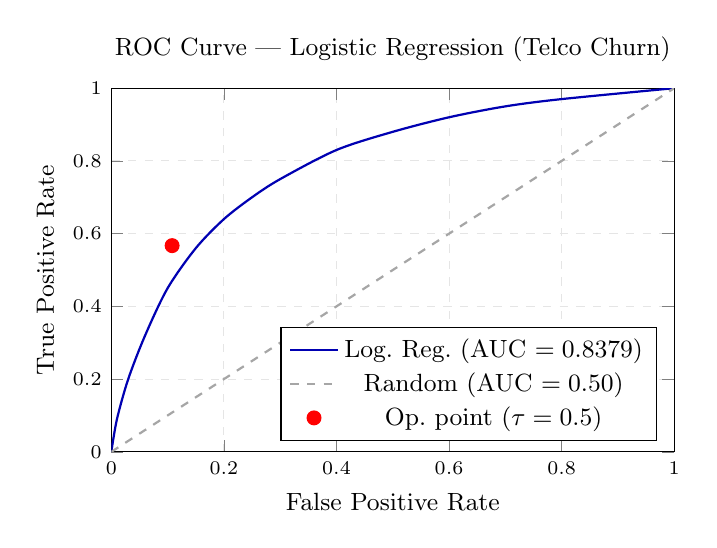
\begin{tikzpicture}
\begin{axis}[
  width=0.72\textwidth, height=6.2cm,
  xlabel={False Positive Rate},
  ylabel={True Positive Rate},
  xmin=0, xmax=1, ymin=0, ymax=1,
  legend pos=south east,
  grid=major, grid style={gray!20, dashed},
  title={\small ROC Curve --- Logistic Regression (Telco Churn)},
  label style={font=\small},
  tick label style={font=\scriptsize},
  legend style={font=\small}
]
\addplot[blue!70!black, thick, smooth] coordinates {
  (0.00,0.00)(0.01,0.09)(0.03,0.20)(0.06,0.32)(0.10,0.45)
  (0.15,0.56)(0.20,0.64)(0.25,0.70)(0.30,0.75)(0.40,0.83)
  (0.50,0.88)(0.60,0.92)(0.70,0.95)(0.80,0.97)(1.00,1.00)
};
\addlegendentry{Log.\ Reg.\ (AUC $= 0.8379$)}
\addplot[gray!70, dashed, thick] coordinates {(0,0)(1,1)};
\addlegendentry{Random (AUC $= 0.50$)}
\addplot[red, mark=*, mark size=2.5pt, only marks]
  coordinates {(0.108, 0.567)};
\addlegendentry{Op.\ point ($\tau=0.5$)}
\end{axis}
\end{tikzpicture}
\caption{ROC curve for the Logistic Regression pipeline.
  The operating point (FPR~$\approx 0.108$, TPR~$\approx 0.567$) marks
  performance at the default 0.5 threshold.}
\label{fig:roc}
\end{figure}

\subsection{Per-Class Analysis}

A marked performance asymmetry exists between the two classes.
The \emph{majority class} (No Churn) achieves Precision $= 0.850$,
Recall $= 0.892$, F1 $= 0.871$---strong, reliable performance.
The \emph{minority class} (Churn) achieves Precision $= 0.656$,
Recall $= 0.567$, F1 $= 0.608$---noticeably weaker, particularly in
recall. This asymmetry directly reflects the 73.4\%/26.6\% class imbalance:
without resampling or cost-sensitive adjustments, the decision boundary
is biased toward the majority class.

% ============================================================
%  6. DISCUSSION
% ============================================================
\section{Discussion}
\label{sec:discussion}

\subsubsection{Accuracy vs.\ Imbalance-Aware Metrics.}
The 80.57\% accuracy is initially encouraging but warrants caution.
A \emph{trivial} classifier predicting ``No Churn'' for every customer
would achieve 73.42\% accuracy, underscoring that accuracy alone is
insufficient for imbalanced evaluation. The more informative results are
the churn-class F1-score (0.608) and the ROC-AUC (0.8379), which confirm
that the model has learned genuine discriminative signal---broadly consistent
with the known prominence of contract type, tenure, and monthly charges
as strong churn predictors~\cite{coussement2008churn}.

\subsubsection{Business Cost Asymmetry and Threshold Tuning.}
The optimal classification threshold $\tau^*$ in a deployment setting
should be derived from the business cost ratio:
\begin{equation}
  \tau^* = \frac{C_{\text{ret}}}{C_{\text{ret}} + LTV}
  \label{eq:tau}
\end{equation}
where $C_{\text{ret}}$ is the cost of a retention offer and $LTV$ is the
customer lifetime value. Lowering $\tau$ below 0.5 increases recall at the
cost of precision---generally the correct trade-off in high-$LTV$ telecom
markets---while the current operating point may be suboptimal for many
commercial scenarios.

\subsubsection{Limitations.}

\begin{description}
  \item[Class Imbalance.] The approximately 2.76:1 majority-to-minority
  ratio biases the decision boundary toward the majority class, depressing
  churn-class recall. Synthetic Minority Over-sampling
  Technique (SMOTE)~\cite{chawla2002smote}, cost-sensitive weighting
  (\texttt{class\_weight=`balanced'}), or threshold calibration represent
  promising remedies.

  \item[Single Hold-out Split.] The single 70/30 stratified split
  produces performance estimates with potentially high variance.
  Stratified $k$-fold cross-validation ($k \in \{5, 10\}$) would yield
  lower-variance, less optimistic generalisation estimates.

  \item[Linear Decision Boundary.] Logistic regression assumes that the
  log-odds of churn are a linear function of the features, and cannot
  directly capture non-linear interactions (e.g., the joint effect of
  Fiber Optic internet \emph{and} a month-to-month contract).
  Gradient Boosted Trees or kernel SVMs may model such interactions
  more effectively.

  \item[Default Hyperparameters.] All hyperparameters were left at their
  scikit-learn defaults ($C = 1.0$, L2 penalty, L-BFGS solver).
  A systematic grid search over $C \in \{10^{-3}, \ldots, 10^{2}\}$
  could materially improve minority-class recall.

  \item[No Feature Importance Analysis.] Although logistic regression
  coefficients provide a form of feature importance after standardisation,
  this analysis was not conducted.
  SHAP (SHapley Additive exPlanations)~\cite{lundberg2017unified} values
  would provide customer-level explanations actionable for retention strategy.
\end{description}

% ============================================================
%  7. CONCLUSION
% ============================================================
\section{Conclusion}
\label{sec:conclusion}

This paper presented a complete, reproducible machine learning pipeline
for binary customer churn prediction on the IBM Telco Customer Churn
dataset. A scikit-learn \texttt{Pipeline} combining median imputation and
standard scaling for numeric features with mode imputation and one-hot
encoding for categorical features was paired with a Logistic Regression
classifier. Evaluated on a stratified held-out test set, the system
achieved 80.57\% accuracy, a churn-class F1-score of 60.80\%, and
ROC-AUC $= 0.8379$, establishing a competitive and interpretable baseline.

Future work should address the five limitations identified in
Section~\ref{sec:discussion}.
Most urgently: (i)~class imbalance mitigation via SMOTE or cost-sensitive
weighting; (ii)~stratified $k$-fold cross-validation for robust performance
estimation; (iii)~model comparison against Random Forest and XGBoost under
identical preprocessing; (iv)~threshold optimisation guided by customer
lifetime value estimates; and (v)~SHAP-based feature importance analysis
to deliver actionable business intelligence alongside predictions.

% ============================================================
%  ACKNOWLEDGEMENTS
% ============================================================
\section*{Acknowledgements}
The author thanks [Instructor Name] for guidance and constructive feedback
on this assignment.
The Telco Customer Churn dataset was sourced from
Kaggle~\cite{kaggle_telco}, originally made available by IBM.

% ============================================================
%  REFERENCES
% ============================================================
\begin{thebibliography}{11}

\bibitem{kaggle_telco}
BlastChar:
Telco Customer Churn (2018).
Kaggle Dataset.
\url{https://www.kaggle.com/datasets/blastchar/telco-customer-churn}

\bibitem{reichheld1990zero}
Reichheld, F.F., Sasser, W.E.:
Zero defections: Quality comes to services.
Harvard Business Review \textbf{68}(5), 105--111 (1990)

\bibitem{coussement2008churn}
Coussement, K., Van den Poel, D.:
Churn prediction in subscription services: An application of support
vector machines while comparing two parameter-selection techniques.
Expert Systems with Applications \textbf{34}(1), 313--327 (2008)

\bibitem{verbeke2012new}
Verbeke, W., Dejaeger, K., Martens, D., Hur, J., Baesens, B.:
New insights into churn prediction in the telecommunication sector:
A profit driven data mining approach.
European Journal of Operational Research \textbf{218}(1), 211--229 (2012)

\bibitem{bhatt2020telco}
Bhatt, P., Bhatt, A.:
Telecommunication customer churn prediction using machine learning.
Procedia Computer Science \textbf{167}, 1270--1276 (2020)

\bibitem{huang2015customer}
Huang, B., Kechadi, M.T., Buckley, B.:
Customer churn prediction in telecommunications.
Expert Systems with Applications \textbf{39}(1), 1414--1425 (2015)

\bibitem{vo2021deep}
Vo, N.N., Liu, S., Li, X., Xu, G.:
Leveraging unstructured call log data for customer churn prediction.
Knowledge-Based Systems \textbf{212}, 106586 (2021)

\bibitem{lariviere2005predicting}
Larivière, B., Van den Poel, D.:
Predicting customer retention and profitability by using random forests
and regression forests techniques.
Expert Systems with Applications \textbf{29}(2), 472--484 (2005)

\bibitem{pedregosa2011scikit}
Pedregosa, F., et al.:
Scikit-learn: Machine learning in Python.
Journal of Machine Learning Research \textbf{12}, 2825--2830 (2011)

\bibitem{chawla2002smote}
Chawla, N.V., Bowyer, K.W., Hall, L.O., Kegelmeyer, W.P.:
SMOTE: Synthetic minority over-sampling technique.
Journal of Artificial Intelligence Research \textbf{16}, 321--357 (2002)

\bibitem{lundberg2017unified}
Lundberg, S.M., Lee, S.I.:
A unified approach to interpreting model predictions.
In: Advances in Neural Information Processing Systems, vol.~30,
pp.~4765--4774. Curran Associates (2017)

\end{thebibliography}

\end{document}